% !TEX root = ../main.tex
%
\chapter{User Study and Evaluation}
\label{sec:study}

To assess the usability and overall utility of the NeRF interface prototype, a comprehensive user study was conducted, which included a variety of tasks to evaluate different aspects of the interface. 
The primary objective of this study was to gather feedback on the prototype's user experience, identify any usability challenges participants encountered, and assess their satisfaction with the interface. 
The use of a mixed-methods approach allowed for the collection and analysis of both quantitative and qualitative data, providing a multifaceted view of the prototype's performance in real-world tasks.

The subjects were then presented with a series of tasks to be completed within the prototype.
Following this, they were asked to complete a User Experience Questionnaire (UEQ) and then participate in a follow-up interview, during which they were encouraged to provide detailed feedback on their experiences.
Of the ten participants, eight studies were conducted in person, while two were conducted remotely due to logistical constraints.

\section{Participant Selection Criteria}
\label{sec:study:criteria}

The participants were selected in a manner analogous to the initial user research phase, with an emphasis on individuals engaged in the film industry and exhibiting a range of experience with NeRF technology, from novices to experts.
The resulting sample was diverse, with participants ranging in experience from those with no prior exposure to NeRF to those with expert-level proficiency \fref{fig:study:experience}.

\begin{figure}[htb]
  \centering
  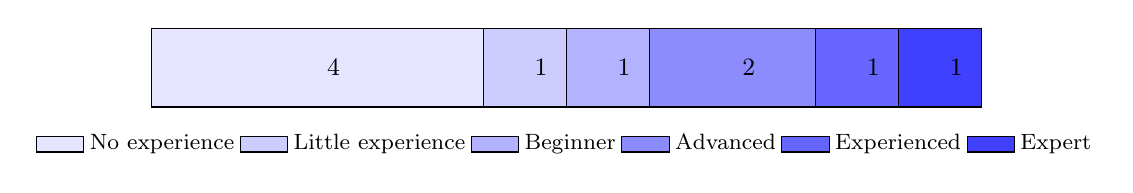
\begin{tikzpicture}
    \pgfplotsset{testbar/.style={
        xbar stacked,
        area style,
        width=\textwidth,
        height=2cm,
        xmajorgrids = false,
        xmin=0, xmax=10, % Adjust max to sum of all values
        ytick=\empty,
        xtick=\empty,
        bar width=15mm,
        y=8mm,
        enlarge y limits={abs=0.625},
        nodes near coords,
        every node near coord/.append style={rotate=0, anchor=west, font=\small}
    }}

    \begin{axis}[testbar,
        legend style={at={(0.5,-0.2)}, anchor=north, legend columns=-1, font=\footnotesize, draw=none}]
        \addplot[fill=blue!10] coordinates{(4,0)};
        \addplot[fill=blue!20] coordinates{(1,0)};
        \addplot[fill=blue!30] coordinates{(1,0)};
        \addplot[fill=blue!45] coordinates{(2,0)};
        \addplot[fill=blue!60] coordinates{(1,0)};
        \addplot[fill=blue!75] coordinates{(1,0)};

        \legend{No experience, Little experience, Beginner, Advanced, Experienced, Expert}
    \end{axis}
  \end{tikzpicture}
  \caption{Level of experience with NeRF technology among participants.}
  \label{fig:study:experience}  
\end{figure}

Four of the participants have backgrounds in filmmaking, including directors, camera operators, and post-production specialists.
The remaining six participants were selected for their expertise in software development and human-computer interaction, as well as their familiarity with NeRF.

\section{Tasks Based Usability Test}
\label{sec:study:tasks}

The usability test was conducted in a controlled environment, where participants were asked to complete a series of tasks with the prototype.
The tasks were designed to cover a range of functionalities and features of the prototype, representing a typical workflow for creating NeRF models.
The tasks included:

\begin{enumerate}
  \item Creating a new project.
  \item Uploading a prepared video file.
  \item Pre-processing the uploaded file to prepare it for training.
  \item Switching to an existing project with pre-processed data.
  \item Starting a NeRF training.
  \item Creating a camera path in the viewer.
  \item Exporting a video.
\end{enumerate}

To maintain an appropriate time frame, none of the tasks required completion of a training process. 
Instead, pre-processed data and pre-trained models were provided.
On average, participants required approximately 30 minutes to complete the tasks.

The participants were observed passively while working on their tasks in order to identify any problems or operational errors they encountered and to determine their overall performance.
Furthermore, the screen was recorded to document the participants' interactions with the prototype, thus enabling a more comprehensive analysis of their behavior at a later stage.

\section{User Experience Questionnaire}
\label{sec:study:ueq}

Once the participants had completed their assigned tasks, they were asked to complete the User Experience Questionnaire (UEQ) \cite{laugwitz_construction_2008}, a standardized tool for assessing user experience.
The UEQ was administered immediately after the tasks to capture the participants' immediate impressions while the experience was still fresh in their minds, and before any influence from the follow-up interview.
Due to an oversight, the UEQ was not administered before the tasks for the studies conducted remotely.

\newpage

The UEQ measures user experience across six dimensions:

\begin{itemize}
  \item \textbf{Attractiveness} - the overall impression of the product.
  \item \textbf{Perspicuity} - the clarity and understandability of the product.
  \item \textbf{Efficiency} - the perceived effort required to use the product.
  \item \textbf{Dependability} - the perceived reliability and trustworthiness of the product.
  \item \textbf{Novelty} - the perceived originality and innovation of the product.
  \item \textbf{Stimulation} - the perceived level of excitement and engagement with the product.
\end{itemize}

This tool covers both classical usability goals (Efficiency, Perspicuity, Dependability) and user experience qualities (Novelty, Stimulation), with Attractiveness serving as a valence dimension not directly related to usability or user experience.

The questionnaire comprises 26 items, each represented by two terms of opposite meaning. The order of the terms is randomized for each item to avoid bias.
Participants are asked to rate each item on a seven-point scale, with values ranging from -3 to +3. The value of 0 represents a neutral response.
An illustrative example of the scale is as follows:

\begin{center}
  \emph{boring} \quad o o o o o o o \quad \emph{exciting}
\end{center}

The participants completed the questionnaire digitally via using a web-based survey tool \cite{noauthor_sosci_nodate}, which also included additional questions to gather demographic information and capture prior experience with NeRF and other 3D modeling tools.

\section{Follow-up Interview}
\label{sec:study:interview}

Following the completion of the usability test, participants were invited to engage in a brief follow-up interview, during which they were encouraged to provide more detailed feedback on their experience with the prototype.
The interviews were semi-structured, following a predefined set of questions, with the option for participants to share their own thoughts and suggestions.
The questions were designed to elicit participants' overall impressions of the prototype, any usability challenges they encountered, and suggestions for improvement.
The interview template is included in the Appendix \ref{sec:appendix:questionnaire}.

\section{Data Analysis}
\label{sec:study:analysis}

Both the video recordings of the usability test and the audio recordings of the follow-up interviews were analyzed to identify common themes and patterns in participant feedback.
The videos were coded to identify usability issues or challenges encountered during tasks, while the interview transcripts were coded to extract detailed feedback and suggestions.

The UEQ data was analyzed using the standard procedure outlined by the questionnaire's authors, which involved the use of a spreadsheet tool for the calculation of all necessary values and the visualization of the results.

In summary, this user study and evaluation served to validate the effectiveness of the NeRF interface prototype, uncover valuable insights into its usability, and identify opportunities for further refinement.
The mixed-methods approach ensured a comprehensive assessment, capturing both the tangible aspects of interface interaction and the subjective experiences of users. This provided a solid foundation for subsequent development stages.
